% !TEX TS-program = pdflatex
% !TEX encoding = UTF-8 Unicode

% This is a simple template for a LaTeX document using the "article" class.
% See "book", "report", "letter" for other types of document.

\documentclass[11pt]{article} % use larger type; default would be 10pt

\usepackage[utf8]{inputenc} % set input encoding (not needed with XeLaTeX)

%%% Examples of Article customizations
% These packages are optional, depending whether you want the features they provide.
% See the LaTeX Companion or other references for full information.

%%% PAGE DIMENSIONS
\usepackage{geometry} % to change the page dimensions
\geometry{a4paper} % or letterpaper (US) or a5paper or....
% \geometry{margin=2in} % for example, change the margins to 2 inches all round
% \geometry{landscape} % set up the page for landscape
%   read geometry.pdf for detailed page layout information

\usepackage{graphicx} % support the \includegraphics command and options

% \usepackage[parfill]{parskip} % Activate to begin paragraphs with an empty line rather than an indent

%%% PACKAGES
\usepackage{booktabs} % for much better looking tables
\usepackage{array} % for better arrays (eg matrices) in maths
%\usepackage{paralist} % very flexible & customisable lists (eg. enumerate/itemize, etc.)
\usepackage{verbatim} % adds environment for commenting out blocks of text & for better verbatim
\usepackage{subfig} % make it possible to include more than one captioned figure/table in a single float
% These packages are all incorporated in the memoir class to one degree or another...

%%% HEADERS & FOOTERS
\usepackage{fancyhdr} % This should be set AFTER setting up the page geometry
\pagestyle{fancy} % options: empty , plain , fancy
\renewcommand{\headrulewidth}{0pt} % customise the layout...
\lhead{}\chead{}\rhead{}
\lfoot{}\cfoot{\thepage}\rfoot{}

%%% SECTION TITLE APPEARANCE
\usepackage{sectsty}
\allsectionsfont{\sffamily\mdseries\upshape} % (See the fntguide.pdf for font help)
% (This matches ConTeXt defaults)

%%% ToC (table of contents) APPEARANCE
\usepackage[nottoc,notlof,notlot]{tocbibind} % Put the bibliography in the ToC
\usepackage[titles,subfigure]{tocloft} % Alter the style of the Table of Contents
\renewcommand{\cftsecfont}{\rmfamily\mdseries\upshape}
\renewcommand{\cftsecpagefont}{\rmfamily\mdseries\upshape} % No bold!

%%% END Article customizations

\usepackage[spanish]{babel}

\usepackage{listings} 

%%% The "real" document content comes below...

\title{JS}
%\date{} % Activate to display a given date or no date (if empty),
         % otherwise the current date is printed 

\begin{document}
\maketitle
%\tableofcontents % No hace falta un TOC en un artículo corto

\section{TUTORIAL DE INSTALACION}
 Desde que los navegadores incluyen el Javascript, no necesitamos el Java Runtime Environment (JRE), para que se ejecute.
\\  \\
Como habilitar JavaScrpt en tu navegador 
Ahora ya todas las páginas web contienen  JavaScript, un lenguaje de programación que se ejecuta en el navegador web del visitante. \\\\
Con esto se crean páginas específicas en las páginas web y si es desactivada o deja de funcionar por cualquier motivo la página web puede verse limitada o no quedar disponible.
\\\\
Veremos como habilitar(activar) JavaScript en cinco de los navegadores mas utilizados:

\section{Google Chrome}


\begin{figure}
\begin{center}
\begin{center}
Navegar google Chrome
\end{center}

\includegraphics[height=3 cm, width=3 cm] {chrome.jpg}

\begin{center}

En el navegador web, haz click en el menú ''Customize and control Google Chrome'' .
y luego selecciona "Settings".
\end{center}

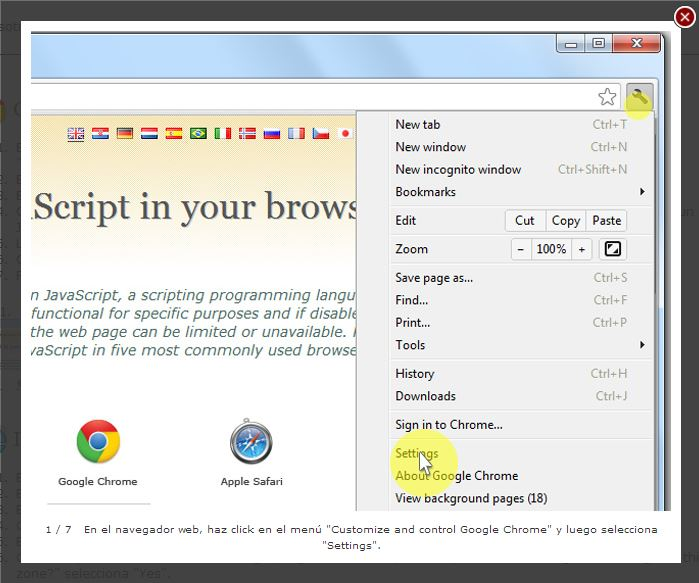
\includegraphics[height=8cm, width=8 cm] {chrome 01.jpg}

\begin{center}
En la sección "Settings" haz click en la 
opción "Show advanced settings..."
\end{center}

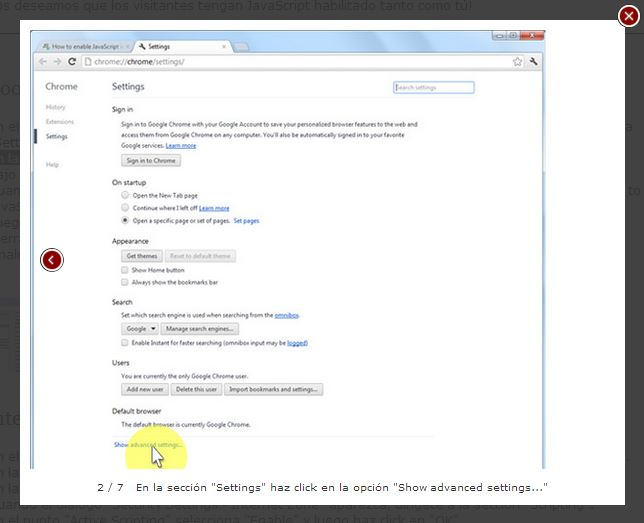
\includegraphics[height=8cm, width=8 cm] {chrome 02.jpg}

\end{center}
\end{figure}

\begin{figure}
\begin{center}
\begin{center}
Bajo la sección "Privacy" haz click en la opción "Content settings...". (recommended)"
\end{center}
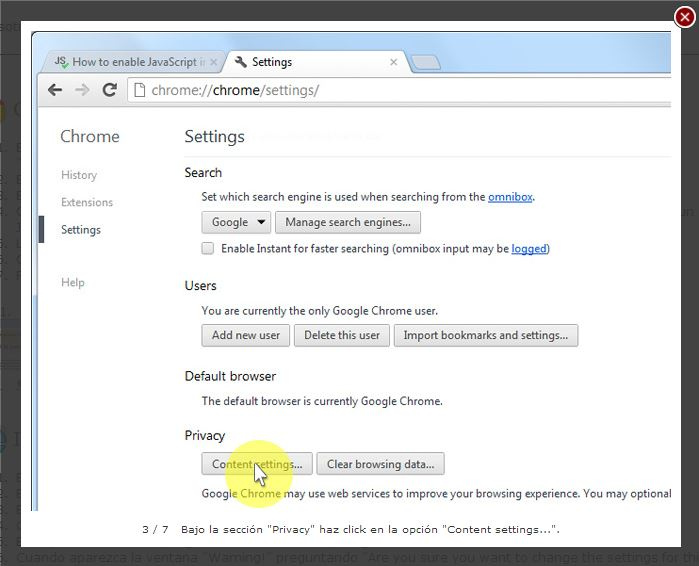
\includegraphics[height=8 cm, width=8 cm] {chrome 03.jpg}

\begin{center}
Cuando la ventana aparezca, dirigirse a la sección "JavaScript" y seleccionar la opción "Allow all sites to run JavaScript (recommended)"
\end{center}

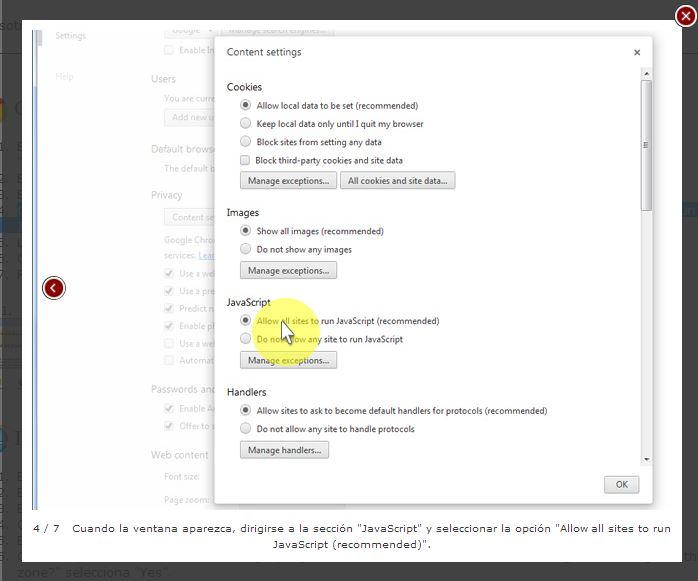
\includegraphics[height=8cm, width=8 cm] {chrome 04.jpg}

\end{center}
\end{figure}

\begin{figure}
\begin{center}
\begin{center}
Luego haz click en el botón "OK" para cerrar la ventana. (recommended)"
\end{center}

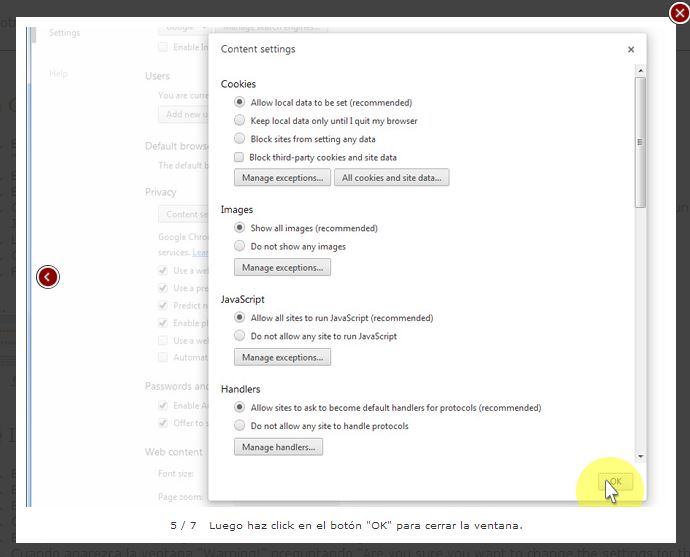
\includegraphics[height=8cm, width=8 cm] {chrome 05.jpg}

\begin{center}
Cierra la pestaña "Settings".
\end{center}

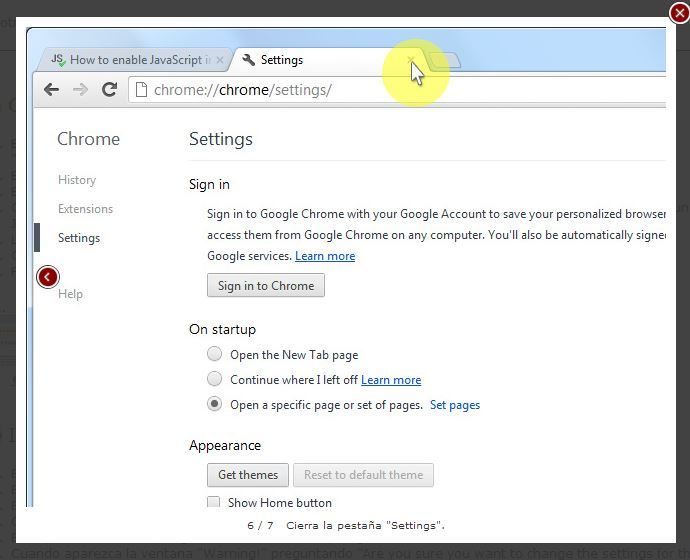
\includegraphics[height=8cm, width=8 cm] {chrome 06.jpg}



\end{center}
\end{figure}


\begin{figure}
\begin{center}
\begin{center}
Finalmente haz click en el botón "Reload this page" del navegador web para refrescar la página.
\end{center}

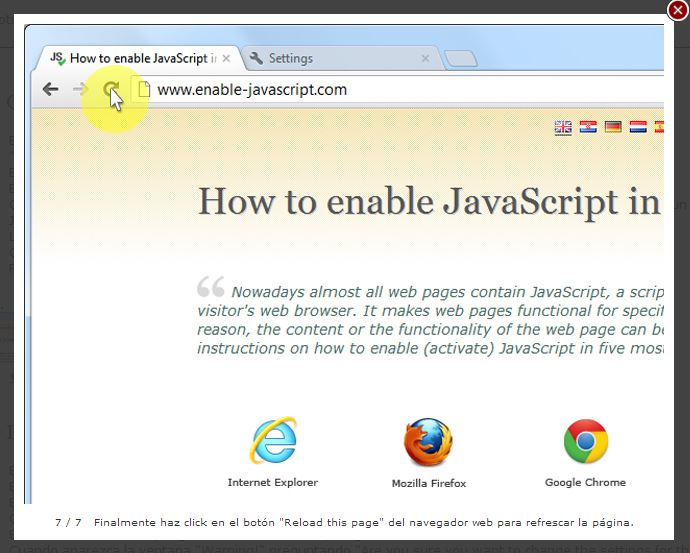
\includegraphics[height=8cm, width=8 cm] {chrome 07.jpg}

\end{center}
\end{figure}

\lstset{language=Pascal}          % Set your language (you can change the language for each code-block optionally)





\end{document}
